% 5 章：合成データによる検証（実験 S1〜S4）
% 数値は results/s1〜s4 の CSV から（memo/09_results_synthetic.md に要約）。
% 表は experiments/s1_recovery.py（tab1_recovery・tab1b_leverage・tab1c_student_t）、s2_agreement.py（tabA2_agreement）、
% s3_scaling.py（tabA3_scaling）、s4_sensitivity.py（tabA1_sensitivity）が生成。図は同じスクリプトが生成（fig2〜fig4、figA1）。
% 付録に回す予定の図表（図A1、表A1〜A3）も、分量の調整までは本章に置いている。
\section{合成データによる検証}\label{sec:synthetic}

本章では、真のパラメータと真のボラティリティが分かっている合成データを使って、\cref{sec:family}の変分族を評価する。
実データでは「正解」が分からないため、推定方法そのものの良し悪しは、まず合成データで確かめておく必要がある。
\cref{sec:syn-overview}で実験の全体像を、\cref{sec:syn-setup}で共通の設定と評価指標を述べる。
\cref{sec:syn-recovery,sec:syn-agreement,sec:syn-scaling,sec:syn-sensitivity}で四つの実験の結果を順に示し、
\cref{sec:syn-summary}で本章の結果をまとめる。

\subsection{実験の目的と全体像}\label{sec:syn-overview}

本章の実験は、次の四つの問いに答えるために設計した。

\begin{enumerate}[label=(Q\arabic*)]
  \item \textbf{真値をどれだけ正確に復元できるか}（実験 S1）。
    多数の合成データについて、パラメータ $\theta$ と潜在ボラティリティ $h_{1:T}$ の推定値が真値にどれだけ近いか、
    95\% 信用区間が名目どおり真値を含むかを調べる。
  \item \textbf{NUTS の事後分布にどれだけ一致するか}（実験 S2）。
    1 本のデータについて、十分に長く回した NUTS を「正解」とし、VI の事後分布の位置と広がりを比べる。
    S1 が「真値との比較」であるのに対し、S2 は「正確なベイズ推定との比較」であり、近似の質そのものを測る。
  \item \textbf{計算時間は系列長 $T$ とともにどう伸びるか}（実験 S3）。
    $T$ を 250 から 10,000 まで変えて、NUTS と VI の所要時間を測る。
  \item \textbf{結果は設定に左右されないか}（実験 S4）。
    パラメータ化（中心化・非中心化）、$\sigma$ の事前分布、ELBO のモンテカルロ（MC）サンプル数、学習率を変えて、推定値が変わるかを調べる。
\end{enumerate}

\cref{tab:syn-design}に各実験の設計をまとめる。
比較する手法は、正解役の NUTS と、\cref{sec:family}の三つの変分族（平均場、構造化、条件付き構造化）を自前の ADVI で最適化したものである。
低ランク・フルランクの族は、\cref{sec:fam-dense}で述べたとおり平均場と同様に崩れるため、S2 で NumPyro の実装を参考として併記するにとどめる。

\begin{table}[tbp]
  \centering
  \caption{合成データ実験の設計。}
  \label{tab:syn-design}
  \footnotesize
  \begin{tabular}{>{\raggedright\arraybackslash}p{0.12\linewidth}>{\raggedright\arraybackslash}p{0.25\linewidth}>{\raggedright\arraybackslash}p{0.24\linewidth}>{\raggedright\arraybackslash}p{0.25\linewidth}}
    \toprule
    実験 & データ & 手法 & 主な評価指標 \\
    \midrule
    S1 復元精度 & 5 シナリオ × $T \in \{500, 2{,}000\}$ × 各 20 本（計 200 本） & NUTS、条件付き構造化（提案）、構造化、平均場 & $\theta$ の偏り・RMSE・95\% 区間の被覆率、$h$ の RMSE・被覆率・sd 比、計算時間 \\
    \addlinespace
    S2 NUTS との一致度 & 高持続シナリオ、$T = 1{,}000$、1 本 & S1 の 4 手法 ＋ NumPyro の 4 ガイド（構造化・平均場・低ランク・フルランク）。NUTS は長い連鎖 & 事後平均、sd 比、Wasserstein 距離、ELBO、$\hat k$、計算時間 \\
    \addlinespace
    S3 計算時間 & 標準シナリオ、$T = 250$〜$10{,}000$ の 6 通り、各 1 本 & NUTS、提案、構造化、平均場（自前・NumPyro） & 所要時間、NUTS の最小 ESS・最大 $\hat R$ \\
    \addlinespace
    S4 設定への感度 & 高持続シナリオ、$T = 1{,}000$、5 本 & 3 族 × 中心化・非中心化、提案手法の事前分布・MC サンプル数・学習率 & 事後平均、NUTS に対する sd 比、収束ステップ \\
    \bottomrule
  \end{tabular}
\end{table}

\subsection{実験設定}\label{sec:syn-setup}

\subsubsection{シナリオとデータの生成}

合成データは、\cref{sec:model}のモデルから直接生成する。
基本 SV モデルについては、持続性の異なる三つのシナリオを用意した。

\begin{itemize}
  \item \textbf{標準}：$\mu = 0$、$\phi = 0.97$、$\sigma = 0.15$。
    日次の株価指数に SV モデルを当てはめたときの典型的な値で、ボラティリティショックの半減期は約 23 日である。
  \item \textbf{高持続}：$\mu = 0$、$\phi = 0.99$、$\sigma = 0.10$。
    ボラティリティの局面が長く続く（半減期は約 69 日）ケースで、隣り合う日の $h_t$ の事後相関がもっとも強い。
    \cref{tab:meanfield-gap}で見たとおり、平均場近似にとってもっとも厳しい設定である。
  \item \textbf{低持続}：$\mu = 0$、$\phi = 0.80$、$\sigma = 0.40$。
    ボラティリティが速く平均に戻る（半減期は約 3 日）ケースである。
    本稿の実データ（1321・1306）の NUTS による推定値は $\phi \approx 0.86$〜$0.89$、$\sigma \approx 0.38$〜$0.46$ であり（\cref{tab:sv-properties}）、
    取得できた期間が約 2 年と短いこともあって、標準シナリオよりもこの低持続シナリオに近い。
\end{itemize}

三つのシナリオは、$h_t$ の定常分布の標準偏差 $s = \sigma / \sqrt{1 - \phi^2}$ がほぼ同じ（0.62〜0.71）になるように選んでいる。
そのため、リターンの尖度や年率ボラティリティの変動幅（\cref{tab:sv-properties}）はシナリオ間でほぼ同じで、違いはボラティリティの「動きの速さ」だけである。
これにより、変分族の性能が持続性 $\phi$ にどう依存するかを、他の要因と切り分けて調べられる。

拡張モデルについては、標準シナリオのパラメータに一つずつ要素を加えた二つのシナリオを用意した。

\begin{itemize}
  \item \textbf{レバレッジ}：標準シナリオに $\rho = -0.5$ を加える（\cref{sec:model-leverage}）。
    日次の株価指数の推定値としてよく報告される水準である。
  \item \textbf{$t$ 誤差}：標準シナリオの誤差を、自由度 $\nu = 8$ の標準化 $t$ 分布にする（\cref{sec:model-t}）。
\end{itemize}

いずれのシナリオでも、$h_1$ は定常分布 $\Normal(\mu, s^2)$ から生成し、その後は\cref{eq:sv-state}に従って $h_2, \dots, h_T$ を生成し、\cref{eq:sv-obs}からリターン $y_t$（\% 単位）を作る。
$\mu = 0$ なので、日次ボラティリティの水準は 1\% 程度（年率で約 16\%）である。
真の平均が 0 のデータなので、実データ（\cref{sec:model-data}）のような標本平均の除去は行わない。
乱数のシードは、実験の番号・シナリオ・$T$・複製の番号から決定的に作り、すべての結果を再現できるようにしている。

\subsubsection{手法の設定}

事前分布は全実験で\cref{tab:priors}の標準の設定を使う（S4 の $\sigma$ の事前分布の比較を除く）。
推定はすべて中心化パラメータ化で行う（S4 のパラメータ化の比較を除く）。
初期値は全手法で共通で、\cref{sec:fam-init}の方法で作る。

\paragraph{NUTS}
NumPyro の NUTS を 4 連鎖で実行する。目標受理率は 0.9 とし、各連鎖の初期値は共通の初期値に小さな乱数（無制約空間で標準偏差 0.1）を加えてずらす。
4 連鎖は CPU の 4 コアで並列に実行する。反復数は実験ごとに次のように変えた。

\begin{itemize}
  \item S1・S4：ウォームアップ 2,000 回、サンプリング 2,000 回（各連鎖。合計 8,000 サンプル）。
    200 本ものデータを推定するため、計算時間と精度の折り合いをつけた長さである。
  \item S2：ウォームアップ 2,000 回の後、32,000 回更新して 8 回に 1 回を保存（各連鎖 4,000 サンプル、合計 16,000 サンプル）。
    VI を評価する「正解」として使うため、十分に長くした。
  \item S3：ウォームアップ 1,000 回、サンプリング 1,000 回。
    実務で「とりあえず回す」ときの長さを想定した。
\end{itemize}

\paragraph{VI}
三つの変分族とも、\cref{sec:inf-advi}の ADVI で最適化する。
最適化手法は Adam で、学習率は 0.01 から始めて最後に 0.001 になるよう指数的に下げる。
ELBO の勾配は、1 ステップあたり $M = 4$ 個の MC サンプルで推定する。
ステップ数は S1・S3・S4 で 10,000、S2 で 20,000 とし、収束したかどうかにかかわらず決められた回数だけ回す（\cref{sec:inf-diagnostics}）。
最適化の後、変分分布から 1,000 個のサンプルを引いて、事後平均や 95\% 区間を計算する。
S2 では、NumPyro の SVI で、平均場（\code{AutoNormal}）、低ランク（\code{AutoLowRankMultivariateNormal}、ランク 10）、
フルランク（\code{AutoMultivariateNormal}）、構造化（自作のガイド）の 4 つも同じステップ数・学習率で最適化した。

\subsubsection{評価指標}

\paragraph{パラメータ}
シナリオ・$T$ ごとに $R$ 本（S1 では $R = 20$）の複製データがあり、$r$ 本目のデータに対する手法の事後平均を $\hat\theta^{(r)}$、
95\% 信用区間（事後分布の 2.5\% 点と 97.5\% 点）を $[\ell^{(r)}, u^{(r)}]$ とする。真値を $\theta^\ast$ とすると、
\begin{equation}
  \begin{gathered}
    \text{偏り} = \frac{1}{R}\sum_{r=1}^R (\hat\theta^{(r)} - \theta^\ast), \qquad
    \mathrm{RMSE} = \sqrt{\frac{1}{R}\sum_{r=1}^R (\hat\theta^{(r)} - \theta^\ast)^2}, \\
    \text{被覆率} = \frac{1}{R}\sum_{r=1}^R \mathbb{1}\{\ell^{(r)} \le \theta^\ast \le u^{(r)}\}
  \end{gathered}
  \label{eq:syn-metrics}
\end{equation}
である。
被覆率は、区間の幅が適切かどうかを測る指標で、名目の 95\% に近いことが望ましい。
被覆率が名目を大きく下回るのは、区間が狭すぎる（不確実性の過小評価）か、区間の位置がずれている（推定の偏り）かのどちらかである。

\paragraph{潜在ボラティリティ}
$h_{1:T}$ については、時点ごとの事後平均の RMSE $\sqrt{T^{-1}\sum_t (\hat h_t - h_t^\ast)^2}$ と、
時点ごとの 95\% 区間が真値を含む割合（時点についての平均）を、データごとに計算して複製で平均する。

注意したいのは、$h_t$ の RMSE は、事後分布を正確に計算できたとしても 0 にはならない点である。
1 日の観測 $y_t$ が $h_t$ について持つ情報は少なく（\cref{sec:model-structure}）、事後分布にはもともと幅がある。
本章の実験では、NUTS でも $h_t$ の RMSE は 0.27（高持続）〜0.53（低持続）である。
このため、$h_t$ の RMSE だけでは手法の差が見えにくく、事後分布の広がりが正しいかを別に調べる必要がある。

\paragraph{NUTS との比較}
VI の事後分布の広がりが正しいかは、NUTS の事後標準偏差との比（\textbf{sd 比}）$\mathrm{sd}_{\mathrm{VI}} / \mathrm{sd}_{\mathrm{NUTS}}$ で測る。
1 なら NUTS と同じ広がり、1 未満なら VI が不確実性を過小評価、1 より大きければ過大評価していることになる。
$h$ については、時点ごとの sd 比の中央値を使う。
S1 では、データごとに sd 比を計算し、複製についての中央値を報告する。

S2 では、さらに次の二つを使う。
一つは、パラメータごとの周辺事後分布の \textbf{1 次元 Wasserstein 距離}で、VI と NUTS のサンプルの分布がどれだけ離れているかを、パラメータと同じ単位で測る。
もう一つは、$h_t$ の\textbf{基準化した平均差} $|\hat h_t^{\mathrm{VI}} - \hat h_t^{\mathrm{NUTS}}| / \mathrm{sd}_{\mathrm{NUTS}}(h_t)$ の時点についての中央値で、
VI の事後平均が NUTS の事後平均から、NUTS の事後標準偏差の何倍ずれているかを表す。
また、ELBO の値（最後の 500 ステップの平均）と PSIS の $\hat k$（\cref{sec:inf-diagnostics}）も報告する。

\paragraph{計算時間}
計算時間は、実行開始から結果が出るまでの経過時間（wall-clock）で測り、JAX の JIT コンパイルの時間を含める。
VI については、二つの時間を区別する。
一つは、決められたステップ数（S1・S3 では 10,000）をすべて実行するのにかかった\textbf{総時間}である。
もう一つは、\textbf{ELBO が収束するまでの時間}で、コンパイル時間に、実行時間を「収束したステップ ÷ 総ステップ数」の割合で按分したものを加えて求める。
収束したステップは、\cref{sec:inf-diagnostics}の判定（200 ステップごとの ELBO の平均の相対変化が $10^{-4}$ を下回った最初の時点）で決める。
前者は「いまの実装で実際にかかった時間」、後者は「収束したところで止めれば、どこまで短くできるか」の目安である。

\paragraph{被覆率の読み方}
S1 の被覆率は 20 本の複製から計算するため、1 本で 0.05 ずつしか変わらない。
真の被覆確率が 0.95 であっても、20 本中の被覆数は二項分布に従ってばらつき、被覆率の標準誤差は $\sqrt{0.95 \times 0.05 / 20} \approx 0.05$ になる。
したがって、0.85〜1.00 程度の被覆率は「名目どおり」と区別できない。
本章で問題にするのは、被覆率が 0.5 を下回るような、統計的なばらつきでは説明できない大きな外れである。

\subsubsection{計算環境}
計算はすべて 1 台のマシン（CPU 12 コア、WSL2 上の Linux、GPU なし）で行った。
ソフトウェアは Python 3.12、JAX 0.12、NumPyro 0.22 で、計算はすべて倍精度（float64）で行う。
VI の最適化は 1 プロセスで実行し、NUTS の 4 連鎖は 4 つの CPU デバイスで並列に実行する。
計時の公平のため、S3 はほかの重い処理と同時に走らせないようにした。

\subsection{真値の復元精度（S1）}\label{sec:syn-recovery}

\cref{tab:recovery}に、基本 SV モデルの三つのシナリオでの結果を示す。
5 シナリオ × 2 通りの $T$ × 20 本 = 200 本のデータを、4 つの手法で推定した（総計算時間は約 5.5 時間）。
表には $\phi$ と $\sigma$ の結果を載せ、$\mu$ については本文で触れる。

\begin{table}[tbp]
  \centering
  \caption{真値の復元精度（S1、基本 SV モデル、各条件 20 本の複製）。
    RMSE と被覆率（95\% 信用区間が真値を含む割合）は\cref{eq:syn-metrics}。
    $h_t$ の RMSE と被覆率は時点について平均したもので、複製で平均している。
    sd 比は、$h_t$ の事後標準偏差の NUTS に対する比（時点についての中央値）の、複製についての中央値。
    時間は JIT コンパイルを含む総時間の中央値（VI は 10,000 ステップ、NUTS は 4 連鎖でウォームアップ・サンプリング各 2,000 回）。}
  \label{tab:recovery}
  \small
  \setlength{\tabcolsep}{4pt}
  \begin{tabular}{llrrrrrrrr}
\toprule
 & & \multicolumn{2}{c}{$\phi$} & \multicolumn{2}{c}{$\sigma$} & \multicolumn{3}{c}{$h_t$} & \\
$T$ & 手法 & RMSE & 被覆 & RMSE & 被覆 & RMSE & 被覆 & sd比 & 時間[s] \\
\midrule
\multicolumn{10}{l}{標準 ($\phi=0.97$)} \\
500 & NUTS (reference) & 0.058 & 0.90 & 0.066 & 0.90 & 0.333 & 0.96 & -- & 11.5 \\
 & VI: conditional (proposed) & 0.054 & 0.85 & 0.054 & 0.90 & 0.332 & 0.95 & 0.95 & 3.2 \\
 & VI: structured & 0.056 & 0.05 & 0.060 & 0.00 & 0.331 & 0.97 & 1.01 & 1.9 \\
 & VI: mean-field & 0.906 & 0.00 & 0.388 & 0.00 & 0.504 & 0.92 & 1.33 & 5.9 \\
2000 & NUTS (reference) & 0.016 & 0.90 & 0.027 & 0.95 & 0.327 & 0.96 & -- & 47.2 \\
 & VI: conditional (proposed) & 0.013 & 0.85 & 0.022 & 0.95 & 0.327 & 0.95 & 0.96 & 11.9 \\
 & VI: structured & 0.028 & 0.10 & 0.057 & 0.00 & 0.333 & 0.97 & 1.09 & 7.3 \\
 & VI: mean-field & 0.938 & 0.00 & 0.399 & 0.00 & 0.559 & 0.92 & 1.46 & 18.6 \\
\midrule
\multicolumn{10}{l}{高持続 ($\phi=0.99$)} \\
500 & NUTS (reference) & 0.045 & 0.90 & 0.064 & 0.80 & 0.270 & 0.98 & -- & 13.4 \\
 & VI: conditional (proposed) & 0.041 & 0.75 & 0.054 & 0.85 & 0.268 & 0.97 & 0.96 & 3.3 \\
 & VI: structured & 0.050 & 0.05 & 0.103 & 0.00 & 0.285 & 0.99 & 1.19 & 1.9 \\
 & VI: mean-field & 0.903 & 0.00 & 0.540 & 0.00 & 0.541 & 0.93 & 1.49 & 5.8 \\
2000 & NUTS (reference) & 0.007 & 0.95 & 0.020 & 0.95 & 0.268 & 0.96 & -- & 73.3 \\
 & VI: conditional (proposed) & 0.006 & 0.85 & 0.017 & 0.95 & 0.268 & 0.95 & 0.97 & 11.9 \\
 & VI: structured & 0.035 & 0.00 & 0.100 & 0.00 & 0.290 & 0.99 & 1.40 & 7.4 \\
 & VI: mean-field & 0.951 & 0.00 & 0.490 & 0.00 & 0.598 & 0.91 & 1.83 & 18.5 \\
\midrule
\multicolumn{10}{l}{低持続 ($\phi=0.80$)} \\
500 & NUTS (reference) & 0.055 & 0.95 & 0.069 & 1.00 & 0.535 & 0.95 & -- & 7.2 \\
 & VI: conditional (proposed) & 0.056 & 0.90 & 0.070 & 1.00 & 0.536 & 0.92 & 0.94 & 3.1 \\
 & VI: structured & 0.107 & 0.00 & 0.166 & 0.00 & 0.545 & 0.84 & 0.75 & 1.9 \\
 & VI: mean-field & 0.721 & 0.00 & 0.273 & 0.00 & 0.613 & 0.93 & 1.10 & 5.7 \\
2000 & NUTS (reference) & 0.036 & 1.00 & 0.046 & 0.95 & 0.521 & 0.94 & -- & 21.2 \\
 & VI: conditional (proposed) & 0.036 & 0.90 & 0.058 & 0.95 & 0.522 & 0.92 & 0.93 & 11.5 \\
 & VI: structured & 0.102 & 0.00 & 0.174 & 0.00 & 0.540 & 0.84 & 0.75 & 7.2 \\
 & VI: mean-field & 0.769 & 0.00 & 0.181 & 0.00 & 0.617 & 0.90 & 1.00 & 18.2 \\
\bottomrule
\end{tabular}

\end{table}

\subsubsection{平均場：持続性 $\phi$ が崩れる}

平均場 VI は、すべてのシナリオ・系列長で $\phi$ の推定に失敗した。
$\phi$ の事後平均は、真値 0.80〜0.99 に対して 20 本の平均で 0.03〜0.09 にとどまり（個々のデータでも最大 0.39）、
RMSE は 0.72〜0.95、被覆率は 0 である。
$T$ を 500 から 2,000 に増やしても改善しない。
これは、\cref{sec:inf-vi}で説明したように、$\phi$ が大きいほど平均場近似の KL の最小値が大きくなり、ELBO が小さい $\phi$ を好むためである。
データを増やしても、$\log p(y \mid \theta)$ と KL の最小値はどちらも $T$ にほぼ比例して増えるので、この偏りは消えない。

$\phi$ が崩れると、ほかのパラメータも引きずられる。
$\phi \approx 0$ の AR(1) では、$h_t$ の日々の変動はすべて $\sigma$ が担うことになるため、$\sigma$ は真値の 0.10〜0.40 に対して 0.52〜0.65 に大きく推定される（偏り $+0.17$〜$+0.50$）。
$h_t$ は日ごとにほぼ独立に推定されるので、ボラティリティの推定値は日々のリターンの大きさに引きずられて激しく上下し、
$h_t$ の RMSE は NUTS の 1.1〜2.2 倍（0.50〜0.62）に悪化する。

注目すべきは、$h_t$ の事後標準偏差がむしろ NUTS の 1.0〜1.8 倍に\textbf{広がっている}ことである。
「平均場近似は事後分散を過小評価する」という一般的な理解（\cref{sec:inf-vi}）とは逆の現れ方であるが、
これは、$\phi$ が崩れたことで、隣り合う日の情報を借りられなくなり、1 日分の観測だけで $h_t$ を決めることになるためである。
$h_t$ の被覆率が 0.90〜0.93 と名目に近いのは、区間が正しいからではなく、中心がずれた分を幅の広さで補っている結果にすぎない。

持続性の低い低持続シナリオ（$\phi = 0.80$）でも、平均場は $\phi$ を 0.03〜0.08 に崩した。
\cref{tab:meanfield-gap}のとおり、$\phi = 0.80$ でも隣り合う日の事後相関は 0.68 あり、KL の最小値は 190 nats に達するため、
平均場の ELBO が小さい $\phi$ を好むことに変わりはない。
つまり、平均場 VI が失敗するのは「持続性が特に高いとき」に限らず、日次の金融データで現実的な範囲のパラメータすべてである。

\subsubsection{構造化：$h$ は良いが、$\sigma$ の不確実性が失われる}

構造化 VI は、$h_t$ の推定では NUTS にかなり近い。
$h_t$ の RMSE は NUTS の 0.99〜1.08 倍にとどまり、標準シナリオでは sd 比も 1.01〜1.09 と NUTS に近い。
三重対角の精度行列で $h_t$ の時間方向の相関を表せる（\cref{sec:fam-structured}の要件 (R1)）ことの効果である。

一方で、$\sigma$ の推定には大きな問題がある。
$\sigma$ の 95\% 区間の被覆率は、すべての条件で 0 である。
$\sigma$ の事後標準偏差は NUTS の 0.07〜0.19 倍しかなく、区間が極端に狭い。
これは\cref{sec:fam-structured}で導いたとおり、$q(h)$ が $\theta$ に依存しない族では、$q(\theta)$ から見ると $h$ の経路がほぼ「観測済み」になり、
$\sigma$ の不確実性が $\sigma / \sqrt{2(T-1)}$ 程度まで縮むためである。
$\phi$ の被覆率も 0〜0.10 と低い。

さらに、$\sigma$ の点推定そのものも偏る。
偏りは標準シナリオで $+0.06$、高持続シナリオで $+0.10$（真値 0.10 の 2 倍）、低持続シナリオでは逆向きの $-0.17$（真値 0.40 に対して約 0.23）である。
$T$ を増やしても偏りは縮まない（$T = 500$ と $2{,}000$ でほぼ同じ）。
偏りの向きがシナリオによって逆になる点は、$h_t$ の sd 比の向きと対応している。
高持続シナリオでは $q(h)$ の幅が NUTS の 1.19〜1.40 倍と広すぎ、$\sigma$ は過大になる。
低持続シナリオでは $q(h)$ の幅が 0.75 倍と狭すぎ（$h_t$ の被覆率も 0.84 に下がる）、$\sigma$ は過小になり、$\phi$ は逆に過大（偏り $+0.10$）になる。
これは、構造化族では $\sigma^2$ が「$q(h)$ の下での経路の増分 $h_{t+1} - \mu - \phi(h_t - \mu)$ の 2 乗の平均」でおおむね決まる（\cref{sec:fam-structured}）こととつじつまが合う。
$q(h)$ の幅が広すぎれば増分のばらつきが大きく見えて $\sigma$ は過大に、狭すぎれば過小になる。
$\theta$ と $h$ が独立な族では、$q(h)$ の幅と $\theta$ の値が ELBO を通じて互いに影響し合い、本来の事後分布の依存（$\sigma$ が大きいほど経路が粗い。\cref{fig:sigma-roughness}）を再現できないまま、別の釣り合いに落ち着く。
どちらの向きに偏るかはデータの性質によるため、実務でこの偏りを補正することは難しい。

\subsubsection{条件付き構造化（提案）：NUTS とほぼ同じ精度}

提案手法は、すべてのシナリオで NUTS とほぼ同じ精度を示した。

\begin{itemize}
  \item \textbf{点推定}：$\phi$・$\sigma$・$h_t$ の RMSE は、6 条件のほとんどで NUTS と同程度か、わずかに小さい。
    たとえば高持続・$T = 2{,}000$ では、$\phi$ の RMSE が NUTS 0.007 に対して 0.006、$\sigma$ が 0.020 に対して 0.017、$h_t$ が 0.268 で同じである。
    $\sigma$ の偏りは $-0.04$〜$+0.04$ で、NUTS（$-0.01$〜$+0.05$）と同程度である。
    低持続・$T = 2{,}000$ の $\sigma$ だけは RMSE が NUTS の 0.046 に対して 0.058 とやや大きく、偏りは $-0.043$ である。
  \item \textbf{区間}：$\sigma$ の被覆率は 0.85〜1.00、$h_t$ の被覆率は 0.92〜0.97 で、いずれも名目どおりと言える。
    $h_t$ の sd 比は 0.93〜0.97 で、NUTS よりわずかに（数 \%）狭いだけである。
  \item \textbf{計算時間}：10,000 ステップを回しきって 3〜12 秒（中央値）で、NUTS（7〜73 秒）の 1/2〜1/6 である。
    実際には ELBO は 1,600〜2,200 ステップ（シナリオごとの中央値）で収束しているので、収束したところで止めればさらに短くなる（\cref{sec:syn-scaling}）。
\end{itemize}

弱点もある。
$\phi$ の被覆率が 0.75〜0.90 と、名目よりやや低い。
$\phi$ の事後標準偏差は NUTS の 0.87〜0.93 倍（複製の中央値）で、区間が 1 割ほど狭いことが原因である。
また、$\mu$ の事後標準偏差は NUTS の 0.56〜0.96 倍と過小で、とくに高持続シナリオで小さい。
これは、$\phi$ が 1 に近いとき、$h$ の水準 $\mu$ がデータからほとんど識別できなくなり、$\mu$ と $\phi$ の事後分布がバナナ型の強い非線形の依存を持つためである。
提案族の $q(u)$ は大域パラメータについて正規分布（フルランクの共分散）なので、線形の相関は表せても、このような曲がった依存は表せない。
もっとも、$\mu$ は年率ボラティリティの「長期的な水準」を決めるパラメータで、VaR などの短期の予測には $h_T$ ほど効かない。
実データでの予測への影響は\cref{sec:empirical}で確かめる。

\subsubsection{系列長 $T$ による違い}

$T$ を 500 から 2,000 に増やすと、NUTS と提案手法では、標準・高持続シナリオの $\phi$ と $\sigma$ の RMSE が半分以下になる（たとえば提案手法の標準シナリオの $\phi$ で 0.054 から 0.013）。
低持続シナリオでは減り方が小さいが（提案手法の $\phi$ で 0.056 から 0.036）、NUTS も同じように減っている。
推定の誤差が統計的な誤差（データの少なさ）で決まっており、近似の誤差は小さいことを示している。
これに対して、平均場と構造化の誤差は $T$ を増やしても減らない。
平均場の $\phi$ の RMSE は 0.906 から 0.938、構造化の高持続シナリオの $\sigma$ の RMSE は 0.103 から 0.100 で、ほとんど変わらない。
データを増やしても消えない誤差は、変分族の表現力の不足による\textbf{系統的な偏り}であり、データ量で解決できる問題ではない。

実データで使える期間（無料プランで約 2 年、$T \approx 480$）は $T = 500$ に相当する。
この長さでは、NUTS でも $\phi$ の RMSE は 0.05 前後あり、パラメータの推定にはもともと大きな不確実性がある。
だからこそ、点推定だけでなく不確実性まで正しく表せることが、実務での推定方法に求められる。

\subsubsection{拡張モデル}

\cref{tab:recovery-leverage,tab:recovery-t}に、レバレッジ SV と $t$ 誤差 SV の結果を示す。

\begin{table}[tbp]
  \centering
  \caption{真値の復元精度（S1、レバレッジ SV、$\mu = 0$、$\phi = 0.97$、$\sigma = 0.15$、$\rho = -0.5$、各条件 20 本）。見方は\cref{tab:recovery}と同じ。}
  \label{tab:recovery-leverage}
  \small
  \setlength{\tabcolsep}{3.5pt}
  \begin{tabular}{llrrrrrrrrrr}
\toprule
 & & \multicolumn{2}{c}{$\phi$} & \multicolumn{2}{c}{$\sigma$} & \multicolumn{2}{c}{$\rho$} & \multicolumn{3}{c}{$h_t$} & \\
$T$ & 手法 & RMSE & 被覆 & RMSE & 被覆 & RMSE & 被覆 & RMSE & 被覆 & sd比 & 時間[s] \\
\midrule
\multicolumn{12}{l}{レバレッジ ($\rho=-0.5$)} \\
500 & NUTS（基準） & 0.029 & 0.90 & 0.051 & 0.85 & 0.149 & 1.00 & 0.324 & 0.95 & -- & 13.4 \\
 & 条件付き構造化（提案） & 0.027 & 0.85 & 0.044 & 0.85 & 0.209 & 0.85 & 0.325 & 0.94 & 0.97 & 5.6 \\
 & 構造化 & 0.040 & 0.25 & 0.071 & 0.00 & 0.212 & 0.20 & 0.333 & 0.97 & 1.09 & 3.9 \\
 & 平均場 & 0.902 & 0.00 & 0.404 & 0.00 & 0.442 & 0.00 & 0.552 & 0.90 & 1.35 & 6.5 \\
2000 & NUTS（基準） & 0.011 & 0.95 & 0.020 & 1.00 & 0.092 & 0.95 & 0.301 & 0.95 & -- & 69.0 \\
 & 条件付き構造化（提案） & 0.012 & 0.85 & 0.020 & 0.95 & 0.145 & 0.35 & 0.303 & 0.95 & 1.01 & 13.3 \\
 & 構造化 & 0.032 & 0.00 & 0.070 & 0.00 & 0.142 & 0.05 & 0.311 & 0.98 & 1.21 & 7.8 \\
 & 平均場 & 0.939 & 0.00 & 0.378 & 0.00 & 0.409 & 0.00 & 0.546 & 0.91 & 1.57 & 20.0 \\
\bottomrule
\end{tabular}

\end{table}

\begin{table}[tbp]
  \centering
  \caption{真値の復元精度（S1、$t$ 誤差 SV、$\mu = 0$、$\phi = 0.97$、$\sigma = 0.15$、$\nu = 8$、各条件 20 本）。見方は\cref{tab:recovery}と同じ。}
  \label{tab:recovery-t}
  \small
  \setlength{\tabcolsep}{3.5pt}
  \begin{tabular}{llrrrrrrrrrr}
\toprule
 & & \multicolumn{2}{c}{$\phi$} & \multicolumn{2}{c}{$\sigma$} & \multicolumn{2}{c}{$\nu$} & \multicolumn{3}{c}{$h_t$} & \\
$T$ & 手法 & RMSE & 被覆 & RMSE & 被覆 & RMSE & 被覆 & RMSE & 被覆 & sd比 & 時間[s] \\
\midrule
\multicolumn{12}{l}{$t$ 誤差 ($\nu=8$)} \\
500 & NUTS (reference) & 0.085 & 0.90 & 0.093 & 0.90 & 11.967 & 0.75 & 0.362 & 0.96 & -- & 22.7 \\
 & VI: conditional (proposed) & 0.075 & 0.65 & 0.074 & 0.95 & 11.340 & 0.60 & 0.359 & 0.95 & 0.95 & 7.6 \\
 & VI: structured & 0.060 & 0.30 & 0.060 & 0.00 & 8.874 & 0.65 & 0.380 & 0.95 & 0.97 & 5.5 \\
 & VI: mean-field & 0.917 & 0.00 & 0.321 & 0.00 & 8.554 & 0.70 & 0.538 & 0.88 & 1.03 & 10.5 \\
2000 & NUTS (reference) & 0.040 & 0.95 & 0.055 & 0.80 & 4.027 & 0.85 & 0.358 & 0.96 & -- & 101.2 \\
 & VI: conditional (proposed) & 0.019 & 0.95 & 0.028 & 0.90 & 3.094 & 0.70 & 0.356 & 0.95 & 0.95 & 14.6 \\
 & VI: structured & 0.034 & 0.05 & 0.060 & 0.00 & 3.537 & 0.05 & 0.462 & 0.93 & 1.14 & 9.1 \\
 & VI: mean-field & 0.955 & 0.00 & 0.235 & 0.00 & 3.175 & 0.05 & 0.642 & 0.73 & 0.97 & 21.4 \\
\bottomrule
\end{tabular}

\end{table}

\paragraph{レバレッジ SV}
$\phi$・$\sigma$・$h_t$ については、基本 SV と同じ傾向である。
平均場は $\phi$ を崩し、構造化は $\sigma$ の被覆率が 0、提案手法は NUTS に近い（$T = 2{,}000$ で $\phi$ の RMSE 0.012、$\sigma$ 0.020、$h_t$ の sd 比 1.01）。

問題は相関 $\rho$ である。
提案手法の $\rho$ は、真値 $-0.5$ に対して 0 の側に偏り（偏りは $T = 500$ で $+0.19$、$T = 2{,}000$ で $+0.13$）、
$T = 2{,}000$ では 95\% 区間の被覆率が 0.35 にとどまる。$\rho$ の事後標準偏差も NUTS の 0.65 倍と狭い。
NUTS の偏りは $T = 2{,}000$ で $+0.001$ なので、これは近似による偏りである。
$T = 2{,}000$ の偏り $+0.13$ は、真値の約 25\% にあたる。
\cref{sec:fam-leverage}で述べたように、真の事後分布では $h_{t+1}$ の条件付き平均に $\rho\sigma y_t e^{-h_t/2}$ という $h_t$ の非線形の項が入るのに対して、
提案族はそれを変分パラメータ $\tilde e_t$ で置き換えた線形の近似で表しているためである。
この偏りは、ステップ数や学習率を変えても変わらなかった。
構造化族も $\rho$ をほぼ同じだけ縮めたうえ（偏り $+0.13$〜$+0.17$）、区間がさらに狭く被覆率は 0.05〜0.20 である。
平均場は $\rho$ もほぼ 0 に崩した（偏り $+0.41$〜$+0.43$）。

レバレッジ効果の符号（$\rho < 0$）と大まかな大きさは提案手法でも捉えられるが、その強さは 2〜3 割控えめに推定される。
$\rho$ の値そのものを使う用途（たとえばボラティリティの非対称な予測）では、この偏りに注意が必要であり、NUTS による確認が望ましい（\cref{sec:system}）。

\paragraph{$t$ 誤差 SV}
提案手法は $\phi$・$\sigma$・$h_t$ について良好である（$T = 2{,}000$ で $\phi$ の被覆率 0.95、$\sigma$ 0.90、$h_t$ の sd 比 0.95）。
ただし $T = 500$ では $\phi$ の被覆率が 0.65 と低い。
このとき $\phi$ の RMSE は NUTS（0.085）より小さい（0.075）ので、区間が狭すぎることが原因である。

自由度 $\nu$ の推定は、NUTS を含むすべての手法で難しい。
$T = 500$ では NUTS でも $\nu$ の RMSE は約 12、偏りは $+10.6$ である。
これは、裾の厚さを決める情報が、数少ない大きなリターンにしか含まれていないためである。
$T = 500$ 程度のデータでは、真値 $\nu = 8$ と事前平均 22（\cref{tab:priors}）の区別がつかず、事後分布は事前分布に強く引っ張られる。
$T = 2{,}000$ でも NUTS の RMSE は 4.0 である。
提案手法の $\nu$ の推定値は NUTS に近いが（$T = 2{,}000$ で偏り $+1.3$、NUTS は $+2.2$）、事後標準偏差は NUTS の 0.58〜0.84 倍と狭めである。
実務的には、2 年程度のデータでは $\nu$ を正確に推定することは期待できず、事前分布の選び方が結果に効くことを念頭に置く必要がある。

\subsubsection{S1 の NUTS の収束について}

最後に、S1 の正解役ではない NUTS 自身の状態にも触れておく。
S1 の NUTS（各連鎖ウォームアップ・サンプリング 2,000 回）では、200 回の推定のうち 156 回で、パラメータの $\hat R$ の最大値が目安の 1.05 を超えた。
パラメータの最小 ESS（8,000 サンプル中）の中央値は 46 にとどまる。
一方、$h_t$ の $\hat R$ の最大値は平均 1.02 で、$h$ の推定には問題がない。発散（divergence）が起きたのは 200 回中 1 回だけである。

これは、中心化パラメータ化の SV モデルで、$\sigma$ と $h$ の強い事後依存のために NUTS の混合が遅くなるという既知の問題（\cref{sec:model-param}）である。
このため NUTS の 95\% 区間の被覆率も 0.80〜1.00 とばらついている。
ただし、上で見た VI の問題（平均場の $\phi$ の崩壊や、構造化の $\sigma$ の被覆率 0）は、NUTS のこの程度の不正確さとは桁違いに大きいので、結論は変わらない。
本稿では、S1 では「真値との比較」を主とし、「NUTS との細かい比較」は十分に長い連鎖を使う S2 で行う。
この結果はまた、「MCMC を使えば常に正確」とは限らず、MCMC にも収束の確認と十分な反復が必要であることを示している（\cref{sec:system}）。

\subsection{NUTS の事後分布との一致度（S2）}\label{sec:syn-agreement}

S2 では、高持続シナリオ（$\phi = 0.99$、$\sigma = 0.10$）から生成した $T = 1{,}000$ のデータ 1 本について、VI の事後分布を NUTS と詳しく比べる。
正解役の NUTS は、4 連鎖で各 34,000 回（ウォームアップ 2,000 回を含む）更新し、178 秒かかった。
パラメータの $\hat R$ の最大値は 1.003、最小 ESS は約 800、$h_t$ の最小 ESS は約 5,000 で、発散はない。
この NUTS の結果は、事後分布の正確な表現とみなしてよい。

\cref{tab:agreement}に数値の要約を、\cref{fig:theta-marginals}にパラメータの周辺事後分布を、\cref{fig:h-bands}に $h_t$ の事後区間を示す。

\begin{table}[tbp]
  \centering
  \caption{NUTS の事後分布との一致度（S2、高持続シナリオ、$T = 1{,}000$）。
    $\phi$・$\sigma$ は事後平均（真値は 0.99・0.10）。
    sd 比は事後標準偏差の NUTS に対する比（$h$ は時点についての中央値）。
    ELBO は最後の 500 ステップの平均、$\hat k$ は PSIS の形状パラメータ（\cref{sec:inf-diagnostics}）。
    時間は JIT コンパイルを含む総時間（VI は 20,000 ステップ）。
    下の 4 行は NumPyro の SVI による。}
  \label{tab:agreement}
  \small
  \setlength{\tabcolsep}{4pt}
  \begin{tabular}{lrrrrrrrr}
\toprule
手法 & $\phi$ & $\sigma$ & $\mathrm{sd}(\phi)$比 & $\mathrm{sd}(\sigma)$比 & $\mathrm{sd}(h)$比 & ELBO & $\hat k$ & 時間[s] \\
\midrule
NUTS (reference) & 0.983 & 0.126 & -- & -- & -- & -- & -- & 178.1 \\
VI: conditional (proposed) & 0.983 & 0.123 & 0.87 & 0.90 & 0.98 & -1579.9 & 0.85 & 7.1 \\
VI: structured & 0.964 & 0.198 & 0.87 & 0.17 & 1.23 & -1586.1 & 1.02 & 3.5 \\
VI: mean-field & 0.053 & 0.703 & 3.57 & 0.56 & 2.11 & -1643.7 & 1.41 & 15.3 \\
VI: structured (NumPyro) & 0.964 & 0.198 & 0.93 & 0.17 & 1.23 & -1586.3 & 1.02 & 17.1 \\
VI: mean-field (NumPyro) & 0.053 & 0.705 & 3.59 & 0.61 & 2.11 & -1643.6 & 1.43 & 20.6 \\
VI: low-rank (NumPyro) & 0.052 & 0.701 & 4.11 & 0.62 & 2.10 & -1643.4 & 1.25 & 43.4 \\
VI: full-rank (NumPyro) & 0.240 & 0.667 & 4.31 & 0.65 & 2.04 & -1705.5 & 4.15 & 229.9 \\
\bottomrule
\end{tabular}

\end{table}

\begin{figure}[tbp]
  \centering
  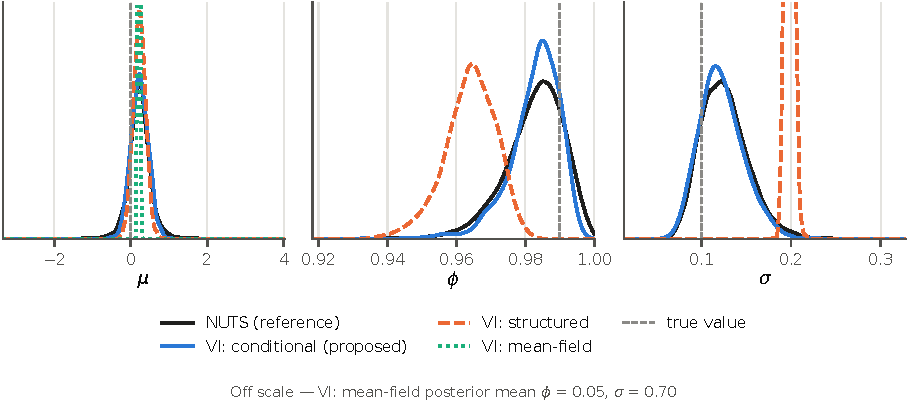
\includegraphics[width=\linewidth]{figures/fig3_theta_marginals.pdf}
  \caption{パラメータの周辺事後分布（S2、高持続シナリオ、$T = 1{,}000$）。
    黒の実線が NUTS（正解）、青の実線が提案手法、橙の破線が構造化、緑の点線が平均場。灰色の縦の破線は真値。
    平均場は $\phi$・$\sigma$ の事後分布が図の範囲外（$\phi \approx 0.05$、$\sigma \approx 0.70$）にある。}
  \label{fig:theta-marginals}
\end{figure}

\begin{figure}[tbp]
  \centering
  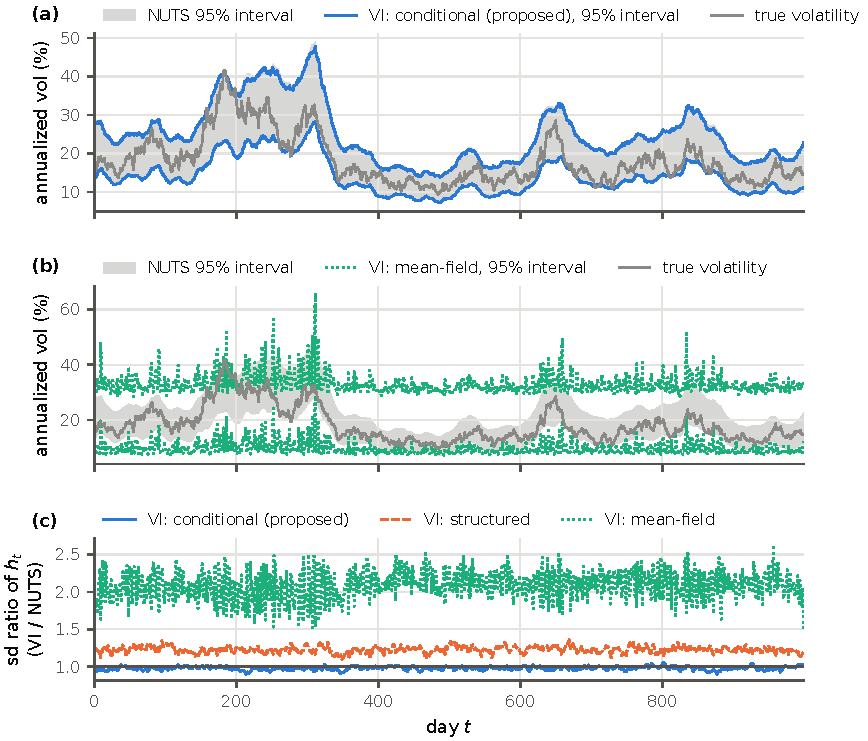
\includegraphics[width=\linewidth]{figures/fig2_h_bands.pdf}
  \caption{潜在ボラティリティの事後区間（S2、高持続シナリオ、$T = 1{,}000$）。
    (a)・(b)：年率ボラティリティ $\sqrt{252}\, e^{h_t/2}$（\%）の 95\% 事後区間。灰色の帯が NUTS、線が VI の区間の上端と下端、灰色の細線が真のボラティリティ。
    (a) は提案手法、(b) は平均場。
    (c)：$h_t$ の事後標準偏差の NUTS に対する比。1 なら NUTS と同じ広がり。}
  \label{fig:h-bands}
\end{figure}

\subsubsection{条件付き構造化（提案）}

提案手法の事後分布は NUTS とよく一致した。
\begin{itemize}
  \item \textbf{パラメータ}：事後平均は $\phi$ が 0.983（NUTS 0.983）、$\sigma$ が 0.123（NUTS 0.126）である。
    \cref{fig:theta-marginals}でも、$\phi$ と $\sigma$ の周辺事後分布は NUTS とほぼ重なる。
    1 次元 Wasserstein 距離は $\phi$ で 0.001、$\sigma$ で 0.003 で、それぞれの事後標準偏差（0.009、0.027）よりも一桁小さい。
    事後標準偏差の比は $\phi$ で 0.87、$\sigma$ で 0.90 で、区間がやや（1 割ほど）狭い。
  \item \textbf{潜在ボラティリティ}：$h_t$ の事後標準偏差の比は中央値 0.98 で、\cref{fig:h-bands}(c) のとおりほぼすべての時点で 1 に近い。
    \cref{fig:h-bands}(a) では、提案手法の 95\% 区間（青線）は NUTS の区間（灰色の帯）の縁にほぼ重なっている。
    事後平均の差は NUTS の事後標準偏差の 0.03 倍（時点の中央値）しかなく、NUTS と見分けがつかない。
  \item \textbf{弱点}：$\mu$ の事後標準偏差は NUTS の 0.66 倍である。
    S1 と同じく、$\phi$ が 1 に近いときの $\mu$–$\phi$ の非線形の依存を表せないためである。
    \cref{fig:theta-marginals}の $\mu$ の図では、NUTS の分布の裾が提案手法より長い。
\end{itemize}

計算時間は、20,000 ステップを回しきって 7.1 秒、ELBO が収束するまで（3,400 ステップ）なら 3.5 秒である。
NUTS（178 秒）と比べると 25〜50 倍速い。

\subsubsection{構造化}

構造化 VI は、$\phi$ の事後平均が 0.964（NUTS 0.983）、$\sigma$ が 0.198（NUTS 0.126）で、とくに $\sigma$ が大きくずれた。
\cref{fig:theta-marginals}の $\sigma$ の図では、構造化の事後分布は $\sigma \approx 0.2$ に鋭く集中し、NUTS の事後分布とほとんど重ならない。
事後標準偏差の比は 0.17 で、\cref{sec:fam-structured}で導いた予測値 $\sigma / \sqrt{2(T-1)} = 0.198 / \sqrt{1998} \approx 0.0044$ は、実際の値 0.0045 とよく一致する。
$\sigma$ の Wasserstein 距離は 0.073 で、提案手法の 20 倍以上である。

$h_t$ については、事後標準偏差の比が 1.23 と広すぎ（\cref{fig:h-bands}(c) の橙の破線）、事後平均の差も NUTS の事後標準偏差の 0.20 倍ある。
$\sigma$ が過大なために、推定されたボラティリティの経路が必要以上に細かく上下していることが原因である。
S1 で見たとおり、構造化 VI の $h_t$ の RMSE は NUTS に近いので、ボラティリティの推定値だけを使う用途では大きな問題にはならないが、
パラメータの不確実性を使う用途（予測分布の幅など）には向かない。

\subsubsection{平均場・低ランク・フルランク}

自前の平均場と NumPyro の平均場（\code{AutoNormal}）は、ともに $\phi \approx 0.05$、$\sigma \approx 0.70$ に崩れた。
\cref{fig:h-bands}(b) では、平均場の 95\% 区間（緑の点線）は日ごとにばらばらに上下し、NUTS の帯から大きく外れている。
上端は年率 30〜40\% 付近、下端は 10\% 付近にほぼ張りついており、ボラティリティの局面の変化をまったく追えていない。
$h_t$ の事後標準偏差は NUTS の約 2 倍（\cref{fig:h-bands}(c)）、事後平均の差は NUTS の事後標準偏差の 1.2 倍である。

パラメータを増やした族も改善しなかった。
ランク 10 の低ランク族（約 12,000 パラメータ）は $\phi = 0.052$、$\sigma = 0.701$ で、平均場とほぼ同じ解に収束した。
フルランク族（約 50 万パラメータ）は 230 秒かけても $\phi = 0.24$、$\sigma = 0.67$ にとどまった。
\cref{fig:elbo}の ELBO の推移を見ると、フルランク族は 20,000 ステップの時点でもまだ ELBO が上昇を続けており、最適化が終わっていない。
\cref{sec:fam-dense}で述べたとおり、パラメータ数を増やすことと、事後分布の構造に合った族を選ぶことは別の問題である。

\subsubsection{ELBO による比較}

\begin{figure}[tbp]
  \centering
  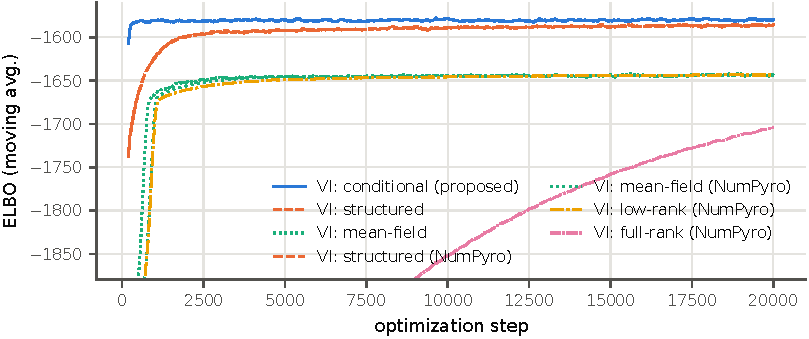
\includegraphics[width=\linewidth]{figures/figA1_elbo.pdf}
  \caption{ELBO の推移（S2、高持続シナリオ、$T = 1{,}000$、200 ステップの移動平均）。
    自前の構造化と NumPyro の構造化の曲線はほぼ重なっている。平均場と低ランクも同じ値に収束する。}
  \label{fig:elbo}
\end{figure}

\cref{fig:elbo}に、最適化中の ELBO の推移を示す。
最終的な ELBO は、提案手法 $-1579.9$、構造化 $-1586.1$、平均場 $-1643.7$、低ランク $-1643.4$、フルランク $-1705.5$ の順である。
ELBO は $\log p(y) - \KL(q \,\|\, p(\cdot \mid y))$ に等しく（\cref{eq:elbo-identity}）、$\log p(y)$ はデータだけで決まって手法によらない。
したがって、ELBO の差はそのまま KL の差であり、提案手法は構造化より約 6 nats、平均場より約 64 nats だけ真の事後分布に近い。
この順位は、パラメータと $h$ の推定の良さの順位と一致している。
同じモデル・同じデータであれば、ELBO を比べることで変分族の良し悪しを判断できる。
これは、実務で変分族や設定を選ぶときの実用的な基準になる（\cref{sec:system}）。

平均場の ELBO が低い値で止まっているのは、最適化が失敗したからではなく、平均場の族の中ではこれが最適だからである。
\cref{tab:meanfield-laplace}で見たように、真の値に近い $\phi$ では平均場近似の KL の最小値が 300 nats を超えるため、
平均場の族の中では、$\log p(y \mid \theta)$ を犠牲にしてでも KL の小さい $\phi \approx 0$ を選ぶ方が ELBO は大きくなる。
平均場の ELBO の曲線は 2,500 ステップほどで平らになっており、最適化そのものは順調に収束している。
「ELBO が収束した」ことは、「事後分布をよく近似できた」ことを意味しないという点は、実務で VI を使ううえで重要な注意点である。

また、自前の構造化と NumPyro の構造化（自作のガイド）は、ELBO（$-1586.1$ と $-1586.3$）・事後平均（$\phi = 0.964$、$\sigma = 0.198$）がともに一致した。
自前の平均場と NumPyro の \code{AutoNormal} も一致している。
独立に書いた二つの実装が同じ結果を出すことは、自前の ADVI の実装の検算になっている。

\subsubsection{PSIS $\hat k$}

$\hat k$ は、提案手法で 0.85、構造化で 1.02、平均場で 1.41、低ランクで 1.25、フルランクで 4.15 であった。
$\hat k$ の大小の順序は近似の良さの順序とおおむね一致するが、提案手法を含むすべての手法で、信頼できる目安とされる 0.7 を超えている。
\cref{sec:inf-diagnostics}で述べたとおり、$\hat k$ は $\theta$ と $h_{1:T}$ をあわせた 1,000 次元を超える同時分布の重要度重みから計算するため、
個々の周辺分布の近似が良くても、高次元での小さなずれが積み重なって大きな値になりやすい。
本稿の結果は、$\hat k$ が「事後分布の同時分布をそのまま重要度サンプリングに使えるか」の基準としては厳しすぎ、
SV モデルの VI の品質の監視には、ELBO の比較や、定期的な NUTS との突き合わせの方が実用的であることを示している（\cref{sec:system}）。

\subsection{計算時間のスケーリング（S3）}\label{sec:syn-scaling}

S3 では、標準シナリオから生成した $T = 250, 500, 1{,}000, 2{,}000, 5{,}000, 10{,}000$ のデータについて、各手法の所要時間を測った。
\cref{fig:scaling}に所要時間を両対数で、\cref{tab:scaling}に数値を示す。
NUTS は 4 連鎖でウォームアップ・サンプリング各 1,000 回の総時間、VI は ELBO が収束するまでの時間である（\cref{sec:syn-setup}）。

\begin{figure}[tbp]
  \centering
  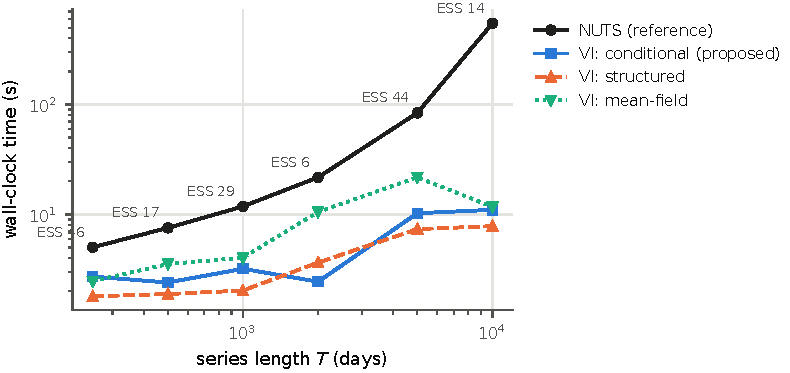
\includegraphics[width=0.88\linewidth]{figures/fig4_scaling.pdf}
  \caption{系列長 $T$ と所要時間（S3、標準シナリオ、両対数）。
    NUTS は 4 連鎖（並列）でウォームアップ・サンプリング各 1,000 回の総時間。VI は ELBO が収束するまでの時間（JIT コンパイルを含む）。
    NUTS の点に添えた数字は、パラメータの最小 ESS（4,000 サンプル中）。}
  \label{fig:scaling}
\end{figure}

\begin{table}[tbp]
  \centering
  \caption{系列長 $T$ と所要時間 [秒]（S3、標準シナリオ）。
    NUTS の時間は総時間、最小 ESS と最大 $\hat R$ はパラメータ $(\mu, \phi, \sigma)$ についての値。
    提案手法は ELBO が収束するまでの時間と、10,000 ステップをすべて実行した総時間の両方を示す。
    ほかの VI は収束するまでの時間。時間はいずれも JIT コンパイルを含む。}
  \label{tab:scaling}
  \small
  \setlength{\tabcolsep}{4pt}
  \begin{tabular}{rrrrrrrrr}
\toprule
 & \multicolumn{3}{c}{NUTS（基準）} & \multicolumn{2}{c}{条件付き構造化（提案）} & \multicolumn{3}{c}{ほかの VI（収束まで）} \\
\cmidrule(lr){2-4} \cmidrule(lr){5-6} \cmidrule(lr){7-9}
$T$ & 時間 & 最小 ESS & 最大 $\hat R$ & 収束まで & 全ステップ & 構造化 & 平均場 & 平均場（NumPyro） \\
\midrule
250 & 5.0 & 46 & 1.04 & 2.7 & 3.0 & 1.8 & 2.5 & 4.2 \\
500 & 7.5 & 17 & 1.53 & 2.4 & 3.0 & 1.9 & 3.5 & 3.7 \\
1,000 & 11.8 & 29 & 1.17 & 3.2 & 4.2 & 2.0 & 4.0 & 8.6 \\
2,000 & 21.7 & 6 & 1.47 & 2.4 & 11.5 & 3.6 & 10.5 & 11.5 \\
5,000 & 83.9 & 44 & 1.04 & 10.3 & 26.0 & 7.4 & 21.8 & 31.1 \\
10,000 & 548.0 & 14 & 1.14 & 11.0 & 52.2 & 7.8 & 11.7 & 29.7 \\
\bottomrule
\end{tabular}

\end{table}

\subsubsection{NUTS}

NUTS の所要時間は、$T = 250$ の 5.0 秒から $T = 10{,}000$ の 548 秒まで、$T$ に比例するよりも速く増えた。
とくに $T = 5{,}000$ から $10{,}000$ では、$T$ が 2 倍になったのに対して時間は 6.5 倍になっている。
NUTS の 1 回の勾配計算は $O(T)$ であるが、次元が大きくなると、事後分布を探索するのに必要なリープフロッグのステップ数（1 回の更新あたりの勾配計算の回数）も増えるためと考えられる。

さらに重要なのは、時間をかけても得られる情報が増えないことである。
パラメータの最小 ESS は、4,000 サンプルに対して 6〜46 しかなく、$T$ によらず小さい（$T = 10{,}000$ で 14）。
$\hat R$ の最大値も 1.04〜1.53 で、6 通り中 4 通りの $T$ で目安の 1.05 を超えている。
つまり、この長さの NUTS の結果は、パラメータについては信頼できる推定とは言えない。
信頼できる結果を得るには、S2 のように連鎖をはるかに長くする必要があり（$T = 1{,}000$ で 178 秒）、所要時間はさらに 1 桁以上増える。
最小 ESS を時間で割った「1 秒あたりの有効サンプル数」は、$T = 250$ の 9.1 から $T = 10{,}000$ の 0.03 まで、約 350 分の 1 に落ちる。

\subsubsection{VI}

提案手法と構造化の VI の所要時間は、$T \le 2{,}000$ では 2〜4 秒でほぼ一定である。
この範囲では、所要時間の大半（約 2 秒）が JIT コンパイルの時間で、最適化そのものは 1 秒程度で終わっている。
$T = 5{,}000$ と $10{,}000$ では、提案手法で約 10〜11 秒になる。
1 ステップの計算量は $O(T)$（\cref{sec:fam-conditional}）なので、10,000 ステップをすべて実行した総時間は $T = 5{,}000$ の 26 秒から $T = 10{,}000$ の 52 秒へと、ほぼ $T$ に比例して増える。
収束までの時間が $T = 5{,}000$ と $10{,}000$ であまり変わらないのは、収束までのステップ数がデータによって 1,800〜3,400 とばらつくためである。

自前実装の平均場と NumPyro の平均場を比べると、NumPyro の方が 1.1〜2.5 倍時間がかかった。
推定結果は同じなので、これは変分族の違いではなく、最適化ループや ELBO の推定のまとめ方といった実装の違いによるものと考えられる。
自前の実装では、最適化のループ全体を一つの関数として JIT コンパイルしている（\cref{sec:system}）。

\subsubsection{速さの比較の読み方}

NUTS と提案手法の速さの比は、どの時間で比べるかによって変わるので、正直に複数の見方を示しておく。

\begin{itemize}
  \item \textbf{収束までの時間で比べる}と、提案手法は $T = 1{,}000$ で約 4 倍、$T = 10{,}000$ で約 50 倍（548 秒に対して 11 秒）速い。
    \cref{sec:intro}の「約 50 倍」はこの比較である。
  \item \textbf{10,000 ステップを回しきった総時間で比べる}と、$T = 1{,}000$ で約 3 倍、$T = 10{,}000$ で約 10 倍（548 秒に対して 52 秒）である。
    収束の判定で自動的に止める実装にすれば前者に、決め打ちのステップ数で回すなら後者に近くなる。
    なお $T = 2{,}000$ では、収束の判定が 800 ステップと早く出ており、収束までの時間（2.4 秒）は総時間（11.5 秒）よりかなり短い。
    収束の判定にはこの程度のばらつきがあるため（その理由は\cref{sec:sys-warm}で述べる）、\cref{fig:scaling}の VI の線の細かい上下は傾向として読むべきである。
  \item \textbf{信頼できる NUTS と比べる}と、差はさらに大きい。
    S3 の NUTS は $\hat R$ が目安を超えており、信頼できる推定には S2 のような長い連鎖が必要になる。
    $T = 1{,}000$ では、S2 の NUTS（178 秒）と提案手法（収束まで 3.5 秒、総時間 7.1 秒）の比は 25〜50 倍である。
\end{itemize}

実データの長さ（$T \approx 480$）で 1 系列だけを推定するなら、NUTS でも数秒〜数十秒で終わり、速さの差は実務上の決め手にならないかもしれない。
VI の速さが効いてくるのは、(i) 系列が長いとき、(ii) 多数の銘柄を一度に推定するとき、(iii) 毎日の再推定のように推定を何度も繰り返すとき、である。
(ii)・(iii) については、実データで\cref{sec:empirical,sec:system}で調べる。

\subsection{設定への感度（S4）}\label{sec:syn-sensitivity}

S4 では、高持続シナリオ（$T = 1{,}000$）のデータ 5 本について、推定の設定を変えたときの結果を比べた。
評価は、各データについて同じ事前分布で回した NUTS（ウォームアップ・サンプリング各 2,000 回）との比で行う。
\cref{tab:sensitivity}に結果を示す。

\begin{table}[tbp]
  \centering
  \caption{設定への感度（S4、高持続シナリオ、$T = 1{,}000$、5 本）。
    $\bar\phi$・$\bar\sigma$ は事後平均の 5 本の平均（真値は 0.99・0.10）、sd 比は NUTS に対する事後標準偏差の比の中央値、
    $h$ の RMSE は真値に対する値の平均、収束 step は ELBO が収束したステップの中央値。
    「中心化」「MC=4」「lr=0.01」は同じ標準の設定を別の乱数で回したものである。}
  \label{tab:sensitivity}
  \footnotesize
  \setlength{\tabcolsep}{3.5pt}
  \begin{tabular}{llrrrrrrr}
\toprule
比較 & 設定 & $\bar\phi$ & $\bar\sigma$ & $\mathrm{sd}(\phi)$比 & $\mathrm{sd}(\sigma)$比 & $\mathrm{sd}(h)$比 & $h$ RMSE & 収束step \\
\midrule
パラメータ化 & meanfield/中心化 & 0.041 & 0.536 & 2.38 & 0.35 & 1.62 & 0.529 & 2600 \\
 & meanfield/非中心化 & 0.039 & 0.555 & 2.32 & 1.35 & 1.70 & 0.528 & 5600 \\
 & structured/中心化 & 0.949 & 0.204 & 0.66 & 0.14 & 1.22 & 0.312 & 3200 \\
 & structured/非中心化 & 0.941 & 0.205 & 0.80 & 0.47 & 1.24 & 0.318 & 2600 \\
 & conditional/中心化 & 0.975 & 0.130 & 0.90 & 0.93 & 0.97 & 0.286 & 1600 \\
 & conditional/非中心化 & 0.975 & 0.129 & 0.90 & 0.87 & 0.97 & 0.285 & 800 \\
\addlinespace
σ の事前分布 & conditional/InvGamma & 0.979 & 0.117 & 0.80 & 0.83 & 0.97 & 0.283 & 1600 \\
\addlinespace
MC サンプル数 & conditional/MC=1 & 0.976 & 0.125 & 0.82 & 0.85 & 0.95 & 0.284 & 5600 \\
 & conditional/MC=4 & 0.975 & 0.129 & 0.92 & 0.92 & 0.98 & 0.285 & 3000 \\
 & conditional/MC=16 & 0.974 & 0.131 & 0.91 & 0.92 & 0.98 & 0.285 & 1800 \\
\addlinespace
学習率 & conditional/lr=0.003 & 0.978 & 0.120 & 0.73 & 0.77 & 0.94 & 0.283 & 2800 \\
 & conditional/lr=0.01 & 0.975 & 0.129 & 0.86 & 0.88 & 0.97 & 0.285 & 2400 \\
 & conditional/lr=0.03 & 0.974 & 0.132 & 0.87 & 0.94 & 0.98 & 0.285 & 1000 \\
\bottomrule
\end{tabular}

\end{table}

\subsubsection{評価そのもののばらつき}

まず、表の数値の読み方として、評価そのもののばらつきの大きさを確かめておく。
表の「条件付き構造化／中心化」「MC=4」「lr=0.01」の 3 行は、いずれも標準の設定（中心化、MC サンプル数 4、学習率 0.01）であり、違うのは最適化の乱数だけである。
この 3 行の間でも、$\sigma$ の sd 比は 0.88〜0.93、$\phi$ の sd 比は 0.86〜0.92、収束ステップは 1,600〜3,000 と変わる。
つまり、sd 比で $\pm 0.05$ 程度、収束ステップで 2 倍程度の違いは、設定の効果ではなく乱数によるばらつきの範囲である。

\subsubsection{パラメータ化}

提案手法は、中心化と非中心化でほぼ同じ結果になった（$\bar\phi = 0.975$ と $0.975$、$\bar\sigma = 0.130$ と $0.129$、$h$ の sd 比はともに 0.97）。
$\sigma$ の sd 比（0.93 と 0.87）の違いは、上のばらつきの範囲に収まる。
これは、\cref{sec:fam-conditional}で示した「提案族はパラメータ化によらず同じ分布の集合になる」という性質を、実験で確かめたものである。
パラメータ化を選ぶ手間（\cref{sec:model-param}）がなくなることは、実務上の利点である。

平均場は、非中心化にしても $\phi \approx 0.04$ に崩れたままであった。
$\sigma$ の sd 比は 0.35 から 1.35 に変わるが、$\phi$ が崩れていることに変わりはない。
平均場の失敗はパラメータ化の問題ではなく、$h_t$ の時間方向の相関を表せないことによる（\cref{sec:inf-vi}）ことが確認できる。

構造化は、非中心化にすると $\sigma$ の sd 比が 0.14 から 0.47 に改善した。
非中心化では $h_t = \mu + \sigma x_t$ と表すので、$q(x)$ が $\theta$ に依存しなくても、$h$ の経路の振れ幅は $\sigma$ に比例して変わる。
つまり、$\sigma$ と $h$ の依存の一部（振れ幅の方向）が、パラメータ化を通じて表されるようになる。
それでも $\sigma$ の sd 比は 0.47 にとどまり、$\bar\sigma$ も 0.205 と過大なままで、提案手法には及ばない。
構造化族では、パラメータ化の選び方で結果が変わり、しかもどちらでも十分ではない。

\subsubsection{$\sigma$ の事前分布}

$\sigma$ の事前分布を、標準の $\mathrm{HalfNormal}(1)$ から、$\sigma^2 \sim \mathrm{InvGamma}(2.5, 0.025)$（事前平均 0.12、95\% 区間 0.06〜0.25。\cref{tab:priors}）に変えると、
提案手法の $\bar\sigma$ は 0.130 から 0.117 に下がり、真値 0.10 に少し近づいた。
これは事前分布が小さい $\sigma$ に情報を持っているためで、NUTS でも同じ方向に動く。
NUTS（同じ事前分布）に対する sd 比は $\phi$ で 0.80、$\sigma$ で 0.83、$h$ で 0.97 で、標準の事前分布のときと大きくは変わらない。
提案手法の近似の質は、事前分布の選び方にはあまり左右されない。

\subsubsection{MC サンプル数と学習率}

ELBO の勾配の MC サンプル数を 1・4・16 と変えても、提案手法の $\bar\phi$（0.974〜0.976）と $\bar\sigma$（0.125〜0.131）はほとんど変わらなかった。
MC サンプル数 1 では sd 比がやや小さく（$\sigma$ で 0.85）、収束ステップが 5,600 と多い。
勾配の雑音が大きいと、最適化に時間がかかり、最終的な変分分布もわずかに狭くなる傾向がある。
1 ステップの計算量は MC サンプル数にほぼ比例するので、本稿の標準の 4 は、精度と計算時間の妥当な折り合いである。

学習率を 0.003・0.01・0.03 と変えた場合も、$\bar\phi$ と $\bar\sigma$ の変化は小さい。
ただし学習率 0.003 では sd 比が $\phi$ で 0.73、$\sigma$ で 0.77 と小さめになった。
学習率が小さいと、10,000 ステップの間に変分分布の広がりの最適化が終わりきらないためと考えられる。
学習率 0.03 では収束が速く（1,000 ステップ）、結果も標準の設定と変わらなかった。
実務で計算時間を短くしたい場合には、学習率を大きめにして早めに打ち切るという選択肢もある。

以上から、提案手法は、パラメータ化・事前分布・最適化の設定のいずれに対しても頑健であり、
設定を細かく調整しなくても安定した結果が得られる。
これは、多数の銘柄を同じ設定で一括して推定する運用（\cref{sec:system}）にとって重要な性質である。

\subsection{まとめ}\label{sec:syn-summary}

本章の合成データ実験の結果をまとめる。

\begin{enumerate}
  \item \textbf{平均場 VI は SV モデルには使えない}。
    持続性 $\phi$ を、真値 0.80〜0.99 に対して 0.03〜0.09 程度（複製の平均）に崩し、$\sigma$ も大きく過大になる。
    データを増やしても、パラメータ化を変えても改善しない。
    低ランク・フルランクの族も同様に崩れる。
    事後分散の過小評価という一般的な問題以前に、点推定そのものが大きく偏る。
  \item \textbf{構造化 VI は $h$ の推定は良いが、$\sigma$ の不確実性を失う}。
    $\sigma$ の 95\% 区間の被覆率は全条件で 0、事後標準偏差は NUTS の 0.07〜0.19 倍で、$\sigma$ の点推定も偏る（偏りの向きはシナリオによって変わる）。
    $\theta$ と $h$ の事後的な依存を表せないことによる。
  \item \textbf{条件付き構造化 VI（提案）は NUTS とほぼ同等の精度を持つ}。
    $\phi$・$\sigma$・$h_t$ の RMSE は NUTS と同程度、$\sigma$ と $h_t$ の区間は名目どおりの被覆率を持ち、
    NUTS の事後分布との比較でも、$h_t$ の事後標準偏差の比は 0.98、事後平均の差は NUTS の事後標準偏差の 0.03 倍である。
    弱点は、$\phi$ の区間がやや（1 割ほど）狭いこと、$\mu$ の不確実性を過小評価すること、レバレッジ SV の $\rho$ を約 25\% 0 の側に縮めることである。
  \item \textbf{提案手法は速い}。
    ELBO の収束までの時間で比べて、$T = 10{,}000$ で NUTS の約 50 倍速く、所要時間は $T$ にほぼ比例して増える。
    NUTS は $T$ とともに時間が超線形に増えるうえ、短い連鎖ではパラメータの混合も不十分である。
    一方、実データの長さ（$T \approx 500$）で 1 系列だけを推定する場合、速さの差は数倍にとどまる。
  \item \textbf{提案手法は設定に頑健である}。
    中心化・非中心化で同じ結果になり、事前分布・MC サンプル数・学習率を変えても結果はほとんど変わらない。
  \item \textbf{ELBO は変分族の良し悪しの比較に使えるが、$\hat k$ は厳しすぎる}。
    同じデータでの ELBO の順位は近似の質の順位と一致した。
    一方、$\hat k$ は提案手法でも 0.85 で、SV モデルの VI の品質監視の主な指標には向かない。
\end{enumerate}

次の\cref{sec:empirical}では、これらの結果が実データでも成り立つかを、日本株の ETF と個別銘柄のデータで確かめる。
とくに、合成データでは確かめられない、モデルの誤特定がある場合の挙動と、VaR の予測という実務上の目的に対する性能を調べる。
